\section{The Overall Approach}
\label{sec:overview}
Loop invariant generation using a guess-and-check approach is an iterative process of \emph{data collection}, \emph{guessing} (i.e., classification in this work) and checking (i.e., verification of the invariant candidate).
%The overall workflow is shown in the Figure~\ref{fig:overview}.
In the following, we present how our approach works step-by-step and illustrate each step with the following example.


\begin{example}
An example Hoare triple is shown in Figure~\ref{fig:running:example:program} (where an \code{assume} statement captures the precondition and an \code{assert} statement captures the postcondition).
The set of variables $V$ contains two integer-type ones: $x$ and $y$. For simplicity, we write $(a, b)$ where $a$ and $b$ are integer constants to denote the  evaluation $\{x \mapsto a, y \mapsto b\}$. Further, we interpret integers in the programs as mathematical integers (i.e., they do not overflow).
%The precondition $\mathit{Pre}$ is $\mathit{x < y}$, which is the same as the loop condition $\mathit{Cond}$.
During each loop iteration, $x$ is increased by $7$ if it is negative (line 4); otherwise, it is increased by $10$ (line 5).
$y$ is decreased by $10$ if it is negative (line 6);
otherwise, it is increased by $3$ (line 7).
The postcondition $Post$ is $y \le x \le y + 16$.
This Hoare triple can be proven using a loop invariant $\mathit{Inv}$: $\mathit{x \le y + 16}$.
In the following, we show how our framework works to learn this loop invariant.
\end{example}
\noindent The overall approach is shown as Algorithm~\ref{alg:active}. We start with randomly generating a set of valuations of $V$, denoted as $SP$, at line 1 (a.k.a.~random sampling). Random sampling provides us the initial set of samples to learn the first classifier.
In this work, we have two ways to generate random samples. One is that we generate random values for each variable in $V$ based on its domain,
assuming a uniform probabilistic distribution over all values in its domain.
The other is that we apply an SMT solver~\cite{barrett2009satisfiability,de2008z3} to generate valuations that satisfy $Pre$
as well as those that dissatisfies $Pre$. These two ways are complementary.
On one hand, without using a solver, we may not be able to generate valuations which satisfy $Pre$ if $Pre$ is very restrictive
(or dissatisfy $Pre$ if the negation of $Pre$ is very restrictive).
On the other hand, using a solver often generates biased valuations. We remark that the cost of generating a random sample is often negligible.

\begin{figure}[t]
\begin{subfigure}{0.5\textwidth}
    \raggedright
    \vspace{0.5cm}
%% {\scriptsize\begin{verbatim}
%% void P(int x, int y) {
%%     assume(x < y);
%%     while (x < y) {
%%         if (x < 0) x = x + 7;
%%         else x = x + 10;

%%         if (y < 0) y = y - 10;
%%         else y = y + 3;
%%     }
%%     assert(x >= y
%%         && x <= y + 16);
%% }
%% \end{verbatim}}
\vspace{-0.2cm} \[
 \begin{array}{ll}
1 & \code{~~~ assume(x~{<}~y);}  \\
2 & \code{~~~ while(x~{<}~y)\{}  \\
3 & \code{~~~ \quad if~(x~{<}~0)~x~{=}~x~{+}~7;}  \\
4 & \code{~~~ \quad else~ x~{=}~x~{+}~10;}\\
5 & \code{~~~ \quad if~(y~{<}~0)~y~{=}~y~{-}~10;} \\
6 & \code{~~~ \quad else~ y~{=}~y~{+}~3;}\\
7 & \code{~~~\}} \\
8 & \code{~~~assert(y~{\leq}~x~{\leq}~y~{+}~16);}
\end{array}
\]
    \vspace{-0.2cm}
    \caption{A sample program}
    \label{fig:running:example:program}
\end{subfigure}%
\begin{subfigure}{.5\textwidth}
      \centering
      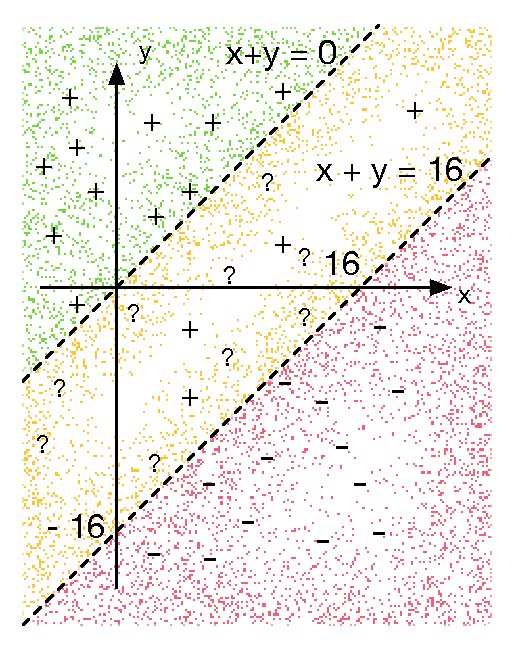
\includegraphics[scale=0.42]{figures/running-sampling.pdf}
      \caption{Sampling}
      \label{fig:running:example:sampling}
\end{subfigure}
\caption{A running example}
\label{fig:running:example}
\end{figure}

\begin{algorithm}[t]
\SetAlgoVlined
\Indm
\Indp
let $SP$ be a set of randomly generated valuations of $V$\;
\While{not time out} {
    call $actL(SP)$ to generate a candidate invariant\;
    \For {each candidate $\phi$} {
        return ``proved'' if the program is verified with $\phi$ otherwise add the counterexample into $SP$\;
    }
}
\caption{Algorithm $zilu()$}
\label{alg:active}
\end{algorithm}

Next, for any valuation $s$ in $SP$, we execute the program starting with initial variable valuation $s$ and record the valuation of $V$ after each iteration of the loop. For any valuation $s$, we write $s \Rightarrow s'$ to denote that there exists $i \geq 0$ such that $s' = Body^i(s)$ and $Body^k(s) \in Cond$ for all $k \in [0, i)$.
That is, if we execute the program with initial valuation $s$, we obtain $s'$ after some number of iterations. We define $SP^*$ to be the set $\{s' | \exists s \in SP.~s \Rightarrow s'\}$. Next, we categorize $SP^*$ into the four disjoint sets: $CE$ (short for counterexample), $Positive$, $Negative$, $NP$. Intuitively, $CE$ contains counterexamples which disprove the Hoare triple; $Positive$ contains those valuations of $V$ which we know must satisfy any loop invariant which proves the Hoare triple; $Negative$ contains those valuations of $V$ which we know must not satisfy any loop invariant which proves the Hoare triple; and $NP$ contains the rest. Formally,
\[
CE(SP) = \{s \in SP^* |~\exists s'.~s \Rightarrow s' \land s \in Pre \land s' \not \in Cond \land s' \not \in Post\} \]
A valuation in $CE(SP)$ satisfies $Pre$ and becomes a valuation $s'$ which fails $Post$ when the loop terminates. If $CE(SP)$ is non-empty, the Hoare triple is disproved.
%\begin{align*}
% \mathit{Positive}(\mathit{SP}) = & \{s | \exists s_0 \in SP.~\exists s'.~s_0 \Rightarrow s' \Rightarrow s \Rightarrow s_n \land \\
%     & ~~~~~~s' \models \mathit{Pre} \land s_n \not \models Cond \land s_n \models \mathit{Post}\}
%\end{align*}
%\begin{align*}
\begin{align*}
Positive(SP) = & \{s \in SP^* | \exists s_0,s_1: SP^*. \\
& ~~~~~~ s_0 \in Pre \land s_0 \Rightarrow s \Rightarrow s_1 \land s_1 \not \in Cond \land s_1 \in Post\}
\end{align*}
$Positive(SP)$ contains a valuation $s$ if there exists a valuation $s_0$ in $SP^*$ which satisfies $Pre$ and becomes $s$ after zero or more iterations. Furthermore, $s$ subsequently becomes $s'$ which satisfies $Post$ when the loop terminates. Let $Inv$ be any loop invariant which proves the Hoare triple. Because $s_0 \in Pre$, $s_0 \in Inv$ since $Inv$ satisfies condition (1). Since $Inv$ satisfies condition (2) and $Body(s_0) \in Inv$ if $Body(s_0) \in Cond$. By a simple induction, we prove $s \in Inv$.
\begin{align*}
    Negative(SP) = & \{s \in SP^* | s \not \in Pre \land \exists s'. \\
    & ~~~~~~s \Rightarrow s' \land s' \not \in Cond \land s' \not \in Post\}
\end{align*}
$Negative(SP)$ is the set of valuations which violates $Pre$ and becomes a valuation $s'$ which violates $Post$ when the loop terminates. We show that $s \not \in Inv$ for all $Inv$ satisfying condition (1), (2) and (3). Assume that $s \in Inv$, by condition (2), $s'$ must satisfy $Inv$ through a simple induction. By condition (3), $s'$ must satisfy $Post$, which contradicts the definition of $Negative(SP)$.
\[    NP(SP) = SP^* - CE(SP) - Positive(SP) - Negative(SP)
\]
$NP(SP)$ contains the rest of the samples. We remark that a valuation $s$ in $NP$ may or may not satisfy an invariant $Inv$ which satisfies condition (1), (2) and (3).

\begin{example}
In our example, assume that the following three valuations are randomly generated:
$(1, 2)$, $(10, 1)$ and $(100, 0)$. Three sequences of valuations are generated after executing the program with these three valuations: $\langle (1, 2), (11, 5) \rangle$, $\langle (10, 1) \rangle$ and $\langle (100, 0) \rangle$.
Note that the loop is skipped entirely for the latter two cases. After categorization, set $CE(SP)$ is empty; $Positive(SP)$ is $\{(1, 2),(11, 5)\}$; $Negative(SP)$ is $\{(100, 0)\}$; and $NP(SP)$ is $\{(10, 1)\}$.
\end{example}
After obtaining the samples and labeling them as discussed above, method $actL(SP)$ at line 4 in Algorithm~\ref{alg:active} is invoked to generate a candidate invariant $\phi$. We leave the details on this method to Section~\ref{sec:classifierlearning}. Once a candidate is identified, we move on to check whether $\phi$ satisfies condition (1), (2) and (3). In particular, we check whether any of the following constraints is satisfiable or not using an $SMT$ solver~\cite{barrett2009satisfiability,de2008z3}.
\begin{align}
    & \mathit{Pre} \land \neg \phi \label{check:inv:pre} \\
     & sp(\phi \land Cond, Body) \land \neg \phi \label{check:inv:loop} \\
    & \phi \land \neg Cond \land \neg Post \label{check:inv:post}
\end{align}
where $sp(\phi \land Cond,Body)$ is the strongest postcondition obtained by symbolically executing program $Body$ starting from precondition $\phi \land Cond$. If all the three constraints are unsatisfiable for any candidate invariant, we successfully prove the Hoare triple. If any of the constraints is satisfiable, a model in the form of a variable valuation is generated, which is then added to $SP$. Afterwards, we restart from data collection, i.e., we execute the program with the counterexample valuations, collect and add the variable valuations after each iteration of the loop to the four categories accordingly, move on to active learning and so on.
\begin{example}
In our example, a candidate invariant which is automatically learned is $x - y \geq 16$. It is easy to check that this candidate satisfies all the three conditions and thus the Hoare triple shown in Figure~\ref{fig:running:example:program} is proved.
\end{example}


